\documentclass[tikz,border=2pt]{standalone}
\renewcommand{\familydefault}{\sfdefault}
\usetikzlibrary{arrows.meta,calc,positioning}
\tikzset{every picture/.style={line width=1pt, >=Stealth},
         hl/.style={fill=black, fill opacity=0.12, text opacity=1}}
\begin{document}
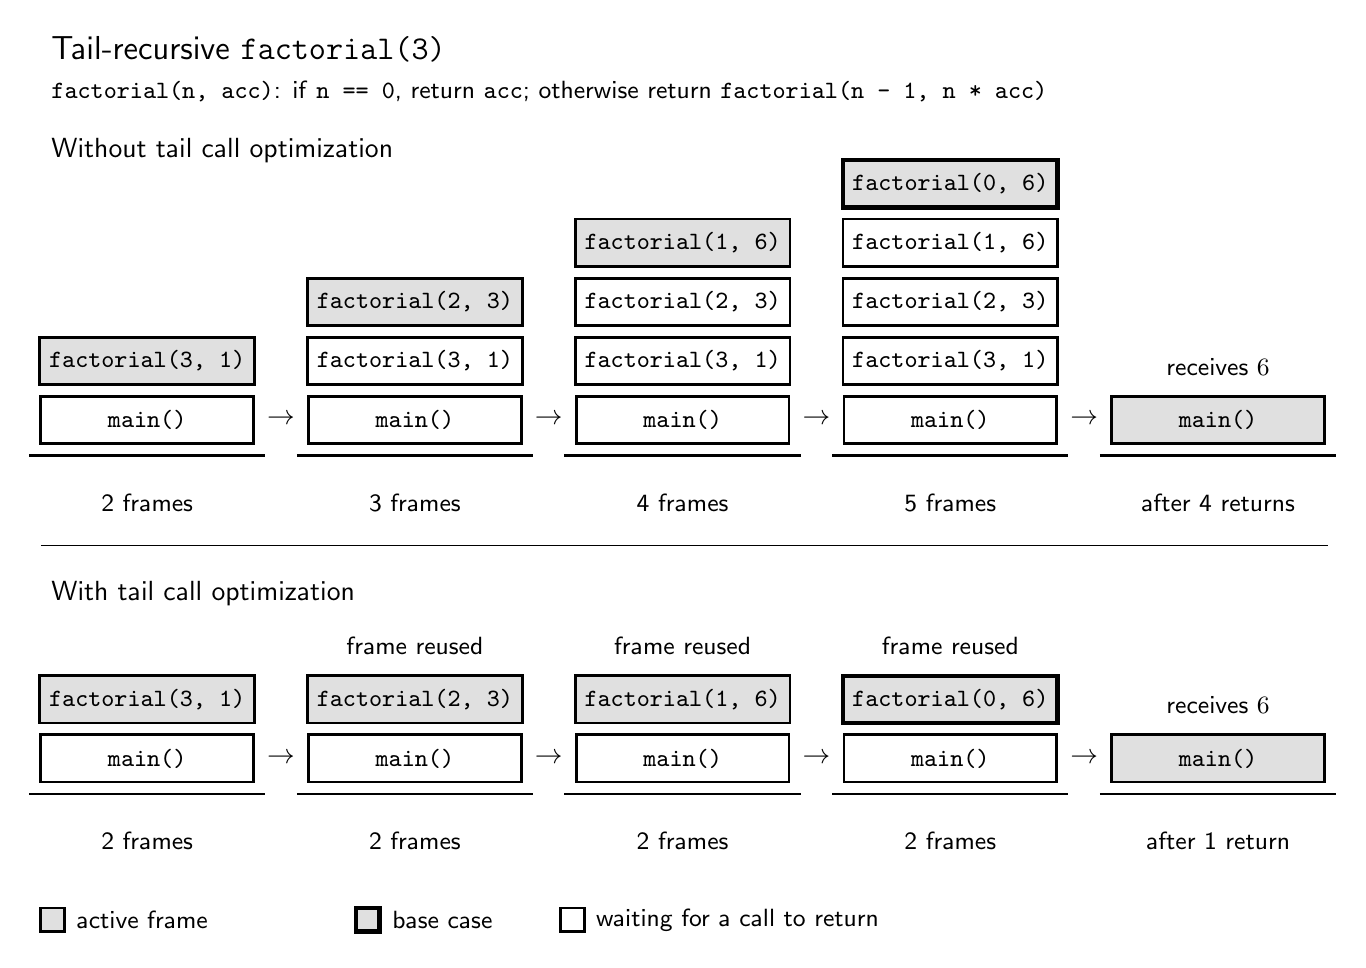
\begin{tikzpicture}[x=1cm, y=0.75cm, frame/.style={draw, minimum width=2.7cm, minimum height=0.6cm, font=\ttfamily\small},
    base/.style={hl, line width=1.6pt}, small/.style={font=\small}]
  % \stack{x}{frame/style, ... from the bottom}{caption}: one snapshot of the call stack
  \newcommand{\stack}[3]{
    \foreach \f/\s [count=\j from 0] in {#2} \node[frame, \s] at (#1, \j) {\f};
    \draw (#1 - 1.5, -0.6) -- (#1 + 1.5, -0.6);
    \node[align=center, small] at (#1, -1.4) {#3};
  }
  \node[anchor=west, font=\large] at (-1.35, 6) {Tail-recursive \texttt{factorial(3)}};
  \node[anchor=west, small] at (-1.35, 5.3) {\texttt{factorial(n, acc)}: if \texttt{n == 0}, return \texttt{acc}; otherwise return \texttt{factorial(n - 1, n * acc)}};
  \node[anchor=west] at (-1.35, 4.3) {Without tail call optimization};
  \begin{scope}[yshift=-0.2cm]
    \stack{0}{main()/, {factorial(3, 1)}/hl}{2 frames}
    \stack{3.4}{main()/, {factorial(3, 1)}/, {factorial(2, 3)}/hl}{3 frames}
    \stack{6.8}{main()/, {factorial(3, 1)}/, {factorial(2, 3)}/, {factorial(1, 6)}/hl}{4 frames}
    \stack{10.2}{main()/, {factorial(3, 1)}/, {factorial(2, 3)}/, {factorial(1, 6)}/, {factorial(0, 6)}/base}{5 frames}
    \stack{13.6}{main()/hl}{after 4 returns}
    \node[small] at (13.6, 0.9) {receives $6$};
    \foreach \x in {1.7, 5.1, 8.5, 11.9} \node at (\x, 0) {$\rightarrow$};
  \end{scope}
  \draw[thin] (-1.35, -2.4) -- (15, -2.4);
  \node[anchor=west] at (-1.35, -3.2) {With tail call optimization};
  \begin{scope}[yshift=-4.5cm]
    \stack{0}{main()/, {factorial(3, 1)}/hl}{2 frames}
    \stack{3.4}{main()/, {factorial(2, 3)}/hl}{2 frames}
    \stack{6.8}{main()/, {factorial(1, 6)}/hl}{2 frames}
    \stack{10.2}{main()/, {factorial(0, 6)}/base}{2 frames}
    \stack{13.6}{main()/hl}{after 1 return}
    \foreach \x in {3.4, 6.8, 10.2} \node[small] at (\x, 1.9) {frame reused};
    \node[small] at (13.6, 0.9) {receives $6$};
    \foreach \x in {1.7, 5.1, 8.5, 11.9} \node at (\x, 0) {$\rightarrow$};
  \end{scope}
  \begin{scope}[yshift=-4.6cm]
  \node[frame, hl, minimum width=0.3cm, minimum height=0.3cm, label=right:{\small active frame}] at (-1.2, -2.6) {};
  \node[frame, base, minimum width=0.3cm, minimum height=0.3cm, label=right:{\small base case}] at (-1.2+4, -2.6) {};
  \node[frame, minimum width=0.3cm, minimum height=0.3cm, label=right:{\small waiting for a call to return}] at (-1.2+6.6, -2.6) {};
  \end{scope}
\end{tikzpicture}
\end{document}
